\section{負荷についての実験}
%%%%%%%%%%%%%%%%%%%%%%%%%%%%%%%%%%
%    実験の目的
%%%%%%%%%%%%%%%%%%%%%%%%%%%%%%%%%%
\subsection{実験の目的}
そこで, Differential Syncronizationに基づいた, 本研究の同期機構が大量のリクエストに対して, どの程度影響が出るか確かめる.
%%%%%%%%%%%%%%%%%%%%%%%%%%%%%%%%%%
%    実験環境
%%%%%%%%%%%%%%%%%%%%%%%%%%%%%%%%%%
\subsection{実験環境}
本手法を実現するサーバとクライアントを実装する. 本実験使用したサーバの計算機環境を表\ref{server}に示す. また2つのクライアントの計算機環境を表\ref{client1}, 表\ref{client2}に示す.
% ネットワーク
\begin{table}[htbp]
\begin{center}
	\caption{使用するサーバのスペック}
	\begin{tabular}{|l|l|} \hline
		OS &  macOS Sierra \\ \hline
		CPU & Intel(R) Core(TM) i5-5250U CPU 1.6GHz \\ \hline
		メモリ & 8GB \\ \hline
    開発言語 & Ruby \\ \hline
		データベース & MySQL \\ \hline
		Webサーバ & Puma\\ \hline
	\end{tabular}
	\label{server}
\end{center}
\end{table}

\begin{table}[htbp]
\begin{center}
	\caption{使用するクライアント1のスペック}
	\begin{tabular}{|l|l|} \hline
		OS & macOS Sierra \\ \hline
		CPU & Intel(R) Core(TM) i5-5250U CPU 1.6GHz \\ \hline
		メモリ & 8GB \\ \hline
    開発言語 & JavaScript HTML \\ \hline
	\end{tabular}
	\label{client1}
\end{center}
\end{table}

\begin{table}[htbp]
\begin{center}
	\caption{使用するクライアント2のスペック}
	\begin{tabular}{|l|l|} \hline
		OS & macOS Sierra \\ \hline
		CPU & Intel(R) Core(TM) i5-5250U CPU 1.6GHz \\ \hline
		メモリ & 8GB \\ \hline
    開発言語 & JavaScript HTML \\ \hline
	\end{tabular}
	\label{client2}
\end{center}
\end{table}

%%%%%%%%%%%%%%%%%%%%%%%%%%%%%%%%%%
%    実験方法
%%%%%%%%%%%%%%%%%%%%%%%%%%%%%%%%%%
\subsection{実験方法}
クライアントを2つ用意した.
クライアント1から命令を発行し, クライアント2の同期レスポンス時間を計測した.
クライアント2がサーバに差分をリクエストした時刻からレスポンスが届いた時刻までを同期レスポンス時間と定義した.
また, クライアントは4秒ごとにサーバにリクエストを送信した.
クライアント1は40秒間4秒ごとに面を作る命令を発行し, 面を作る命令の数を4秒ごとに倍にしていった.
その間, クライアント2では同期レスポンス時間の計測を行なった.
%%%%%%%%%%%%%%%%%%%%%%%%%%%%%%%%%%
%    実験結果
%%%%%%%%%%%%%%%%%%%%%%%%%%%%%%%%%%
\subsection{実験結果}
クライアント2での同期レスポンス時間の計測した結果を図\ref{jikken3}に示す.
項目は左から送信するデータの大きさ, 同期レスポンス時間, 同期レスポンス時間を表したタイムラインである. 計測の結果, 命令の数が増えるとデータの大きさが大きくなり, 同期にレスポンス時間が増える.
\begin{figure}[htbp]
 \begin{center}
	 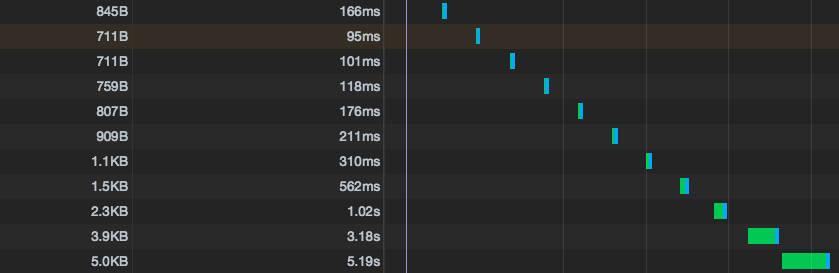
\includegraphics[scale=0.5]{images/jikken3}
	 \caption{クライアント2での同期レスポンス時間}
	 \label{jikken3}
 \end{center}
\end{figure}


%%%%%%%%%%%%%%%%%%%%%%%%%%%%%%%%%%
%    考察
%%%%%%%%%%%%%%%%%%%%%%%%%%%%%%%%%%
\subsection{考察}
結果より, 面を作る数が増え, 一度に大量の編集命令がサーバにリクエストされた場合, サーバでの適用や差分の計算に要する時間が多くかかり遅延が生まれてしまっていた.
原因として, データベースでの挿入や検索がボトルネックになっていると考えられる.
